\section{High level components and their interaction}
\paragraph{}We can sketch our system like in figure \ref{fig:architectureOverview}
\begin{figure}
	\centering
	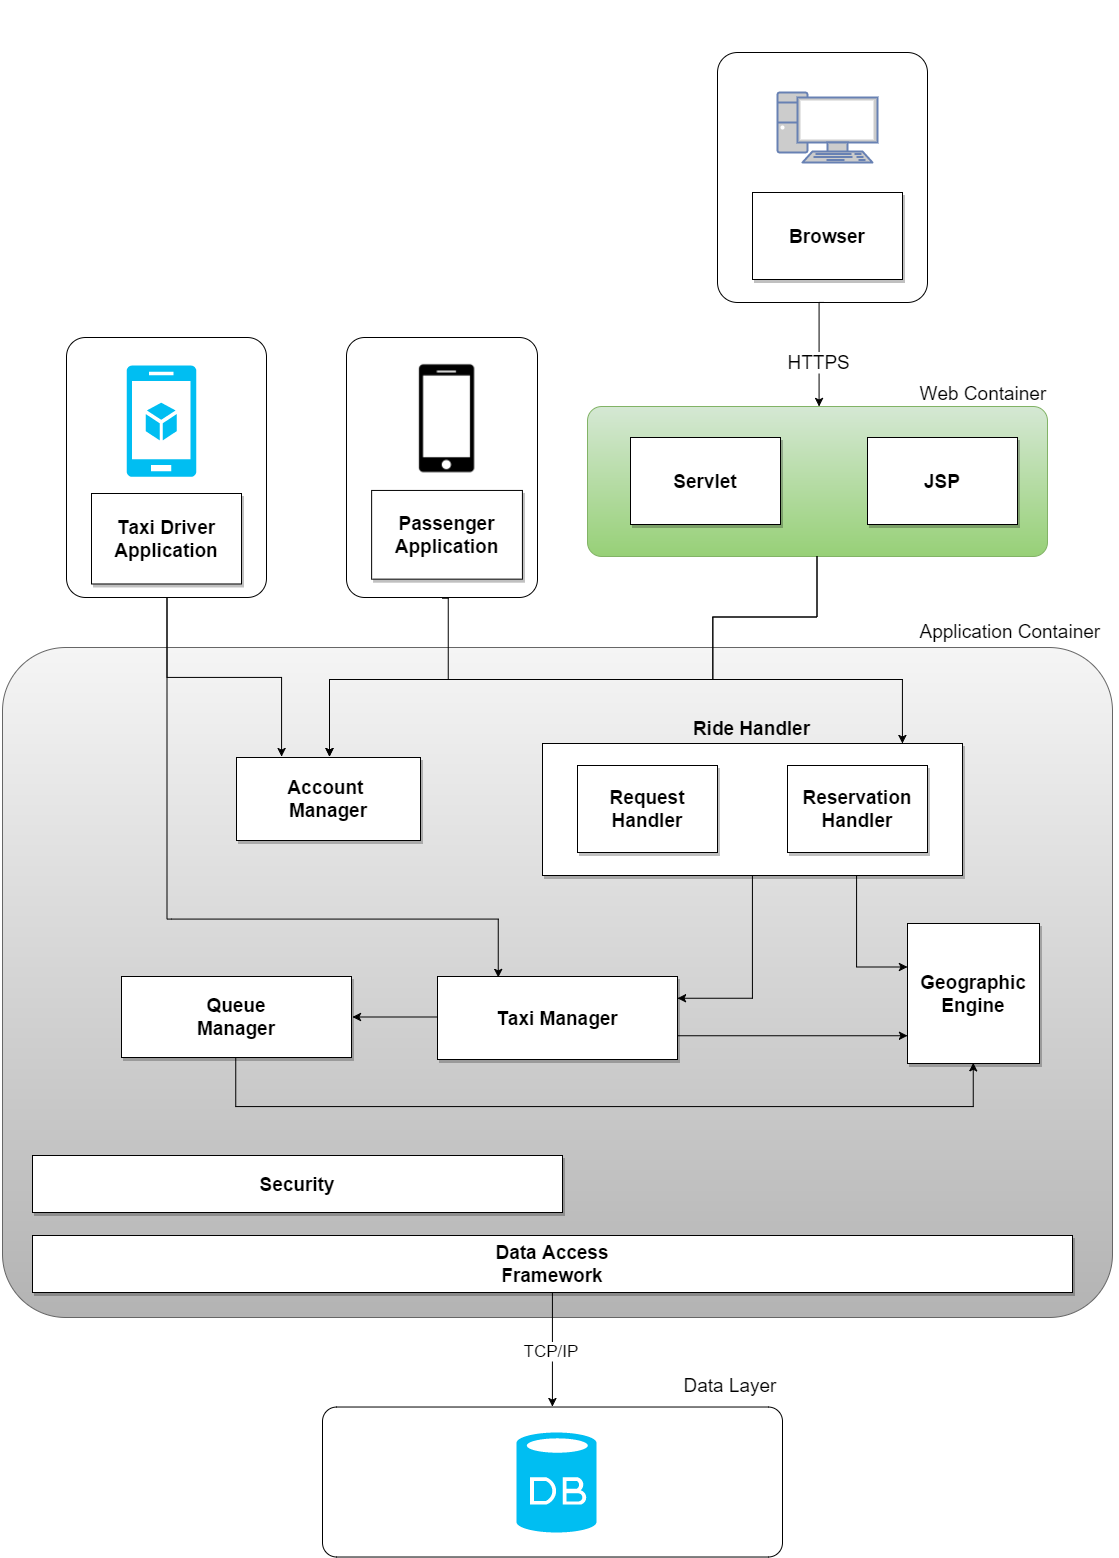
\includegraphics[trim= 0 0 0 200,scale=0.4]{../"Analysis Documents"/ArchitectureOverview.png}
	\caption{Architecture Overview}
	\label{fig:architectureOverview}
\end{figure}
\paragraph{}Here we can see the different components, both hardware and software, and how they are interconnected from a very high point of view.
\paragraph{} In particular the web browser will interface the business logic through a web server, which implements services like Servlets and JSP. In this case, so, the chosen protocol will be HTTPS.\\
As far as mobile applications are concerned they will interface the system through remote calls.
\paragraph{}The application server will be divided in software components differentiated by their role in the implementation of the business logic. For data access and security will be used ready-made components provided by the JEE infrastructure.
\paragraph{} The application server and the data layer will communicate through a TCP/IP connection.
\subsection{Business logic components}
\paragraph{} In figure \ref{fig:highLevelComponents} we find an overview of the business logic components of our application.
\begin{figure}
	\centering
	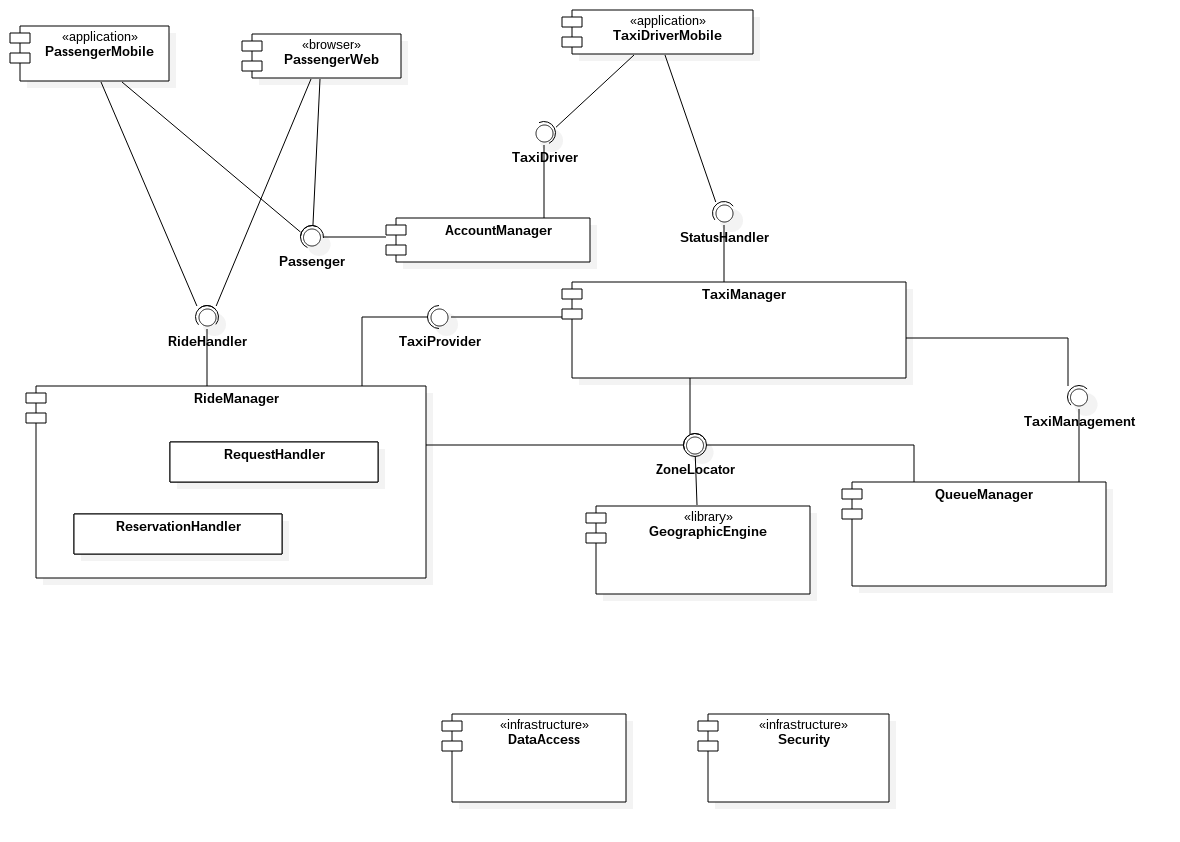
\includegraphics[trim=0 0 150 0, angle=90,scale=0.55]{../"Analysis Documents"/highLevelComponents.png}
	\caption{High level components of the business logic}
	\label{fig:highLevelComponents}
\end{figure}

\begin{enumerate}
	\item \textbf{Account Manager}: It manages the accounts, both of Passengers and Taxi Drivers. It also handles the login and logout phases of both users and the registration for the Passenger and the relative account deleting. It exposes the following interfaces:
	\begin{itemize}
		\item \texttt{Passenger}: for the interaction with the Passengers
		\item \texttt{Taxi Driver}: for the interaction with the Taxi Drivers
	\end{itemize}
	\item \textbf{Ride Manager}: this component is delegated to the management of the life cycle of the incoming requests and reservations from the passengers. From this point of view it can be divided in two main subcomponents:
	\begin{itemize}
		\item \textit{Request Handler}
		\item \textit{Reservation Handler}
	\end{itemize}
	It exposes the following interfaces:
	\begin{itemize}
		\item \texttt{RideHandler}: which can be used by the Passenger mobile application and the web browser (web server)
	\end{itemize}
	\item \textbf{Taxi Manager}: manages the life cycle of the taxi drivers, starting from the availability status and the retrieving of their location. It is in charge of forward to the taxi drivers the calls from the passengers.\\ It exposes the following interfaces:
	\begin{itemize}
		\item \texttt{StatusHandler}: to communicate with the Taxi driver
		\item \texttt{TaxiProvider}: to communicate with the RideManager
	\end{itemize}
	\item \textbf{Queue Manager}: it is in charge of the management of the taxi queues in the different zones of the city, applying the decided policy.\\
	It exposes the following interfaces:
	\begin{itemize}
		\item \texttt{TaxiManagement}: to communicate with the TaxiManager
	\end{itemize}
	\item \textbf{Geographic Engine}: the roles of this component are to implement the algorithms to calculate the zone corresponding to a particular location. It is also in charge of the geographic definition of the taxi zones.\\It exposes the following interfaces:
	\begin{itemize}
		\item \texttt{ZoneLocator}: which provides calculations methods to the other components
	\end{itemize}
	\item \textbf{Security}: a ready-made software component to ensure the safety of tcp/ip connections from the mobile devices and from the web browser
	\item \textbf{Data Access}: framework that abstracts the underlying database logic and enables to map the business logic entities into tables.6
\end{enumerate}